\documentclass[12pt]{article}

\usepackage{sbc-template}

\usepackage{graphicx,url}
\usepackage{placeins}
\usepackage{float}


\usepackage[brazil]{babel}
\usepackage[utf8]{inputenc}

\usepackage{algorithm}
\usepackage{algpseudocode}

\usepackage{booktabs}
\newcommand{\tra}[1]{\renewcommand{\arraystretch}{#1}}

\sloppy

\title{Reutilização de Software -- Documentação do Trabalho Prático}
%\subtitle{Um Servidor de Jogos para Ensino de Engenharia de Software}

\author{Danilo Ferreira e Silva\inst{1}}


\address{Departamento de Ciência da Computação -- UFMG
  \email{danilofs@dcc.ufmg.br}
}

\begin{document} 

\maketitle



\section{Introdução}

Jogos didáticos são instrumentos de apoio ao ensino utilizados em diversas áreas do conhecimento. Especificamente, na área de Engenharia de Software, podemos citar como exemplos os jogos \emph{Programs And Programmers} \cite{baker2005pnp} e \mbox{\emph{SimulES}} \cite{figueiredo2007simules}. O trabalho proposto na disciplina tem como objetivo projetar e implementar um sistema, empregando as técnicas vistas em aula, que se enquadre no tema de jogos para ensino de Engenharia de Software.
Alinhado a esses objetivos, este documento descreve o projeto e implementação de um servidor de jogos extensível, na forma de uma Linha de Produtos de Software (SPL).
%, com suporte para o jogo \emph{SimulES} e um jogo de perguntas e respostas.

O restante deste documento está organizado da seguinte forma. Na Seção~\ref{sec:requisites}, apresentamos a visão geral do sistema e o conjunto de características da SPL. Na Seção~\ref{sec:design}, apresentamos as principais decisões de projeto, incluindo o cronograma de atividades, as técnicas utilizadas, a arquitetura adotada e padrões de projeto empregados. Finalmente, na Seção~\ref{sec:examples} detalhamos como gerar e executar um produto, usando como exemplo duas configurações de características diferentes.


\section{Sistema Proposto}
\label{sec:requisites}

O sistema projetado, que foi denominado SEGE, é um serviço Web de jogos. O sistema consiste de um núcleo e um ou mais jogos, desenvolvidos como \emph{plug-ins}. No contexto deste trabalho, foram incluídos dois jogos: \emph{SimulES} e um jogo de perguntas e respostas baseado nas aulas virtuais da disciplina (\emph{Quiz}). No entanto, novos jogos podem ser desenvolvidos desde que eles: (i) sejam baseados em turnos e (ii) em cada turno exista um conjunto finito de ações, que possam ser mapeadas em uma string.

Além do serviço, a SPL inclui um cliente simples, baseado em linha de comando, utilizado para testar o produto. Embora uma interface gráfica Web seja desejável, optamos por não incluí-la no escopo do trabalho por questões de prazo.

A Figura~\ref{img:feature-model} apresenta o modelo de características (\emph{feature model}) da SPL. Além disso, a Tabela~\ref{tab:features} descreve de forma sucinta cada característica do modelo. É importante ressaltar que, além do modelo prever a customizar do protudo pela inclusão/exclusão de jogos, cada jogo também apresenta variabilidade. Por exemplo, o banco de perguntas do jogo \emph{Quiz} pode ser customizado para incluir temas como Arquitetura de Software, Idiomas de Programação, Desenvolvimento Orientaçdo a Aspectos, etc.

\begin{figure}[htb]
\centering
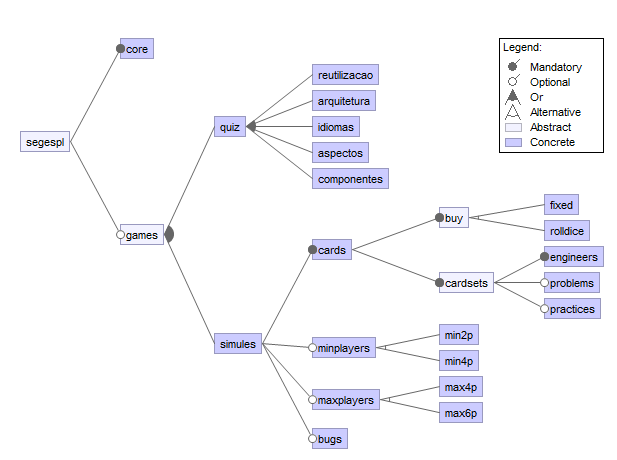
\includegraphics[width=0.8\textwidth]{img/features.png}
\caption{Modelo de características (\emph{feature model})}
\label{img:feature-model}
\end{figure}


\begin{table*}[htb]\centering
\footnotesize
\tra{1.1}
\begin{tabular}{@{}ll@{}}\toprule
\textbf{Característica} & \textbf{Descrição} \\
\midrule
core & Núcleo do sistema, incluindo o serviço Web \\
console\_client & Cliente simples em linha de comando \\
games & Define os jogos disponíveis\\
quiz & Jogo de perguntas e respostas baseado no \emph{quiz} das aulas virtuais\\
questions\_reuse & Conjunto de perguntas de Reutilização de Software\\
questions\_architecture & Conjunto de perguntas de Arquitetura de Software e Padrões Arquiteturais\\
questions\_idioms & Conjunto de perguntas de Idiomas de Programação\\
questions\_aspects & Conjunto de perguntas de Desenvolvimento Orientado a Aspectos\\
questions\_cbse & Conjunto de perguntas de CBSE\\
simules & Jogo SimulES\\
card\_buy\_strategy & Define a estratégia de compra de cartas\\
fixed & Compra um número fixo de cartas por turno\\
rolldice & Compra um número de cartas por turno de acordo com o lançamento de um dado\\
card\_sets & Conjunto de cartas disponíveis\\
engineers & Cartas de engenheiros de software\\
problems & Cartas de problemas\\
practices & Cartas de práticas de Engenharia de Software\\
bugs\_8p & Habilita a existência de bugs\\
min\_players & Habilita a regra de mínimo de jogadores\\
min\_2p & Mínimo de dois jogadores\\
min\_4p & Mínimo de quatro jogadores\\
max\_players & Habilita a regra de máximo de jogadores\\
max\_6p & Máximo de seis jogadores\\
max\_8p & Máximo de oito jogadores\\
\bottomrule
\end{tabular}
\caption{Descrição das características}
\label{tab:features}
\end{table*}


\FloatBarrier
\section{Projeto}
\label{sec:design}

O sistema foi projetado e desenvolvido utilizando uma metodologia semelhanto ao modelo cascata. O planejamento do projeto incluiu cinco atividades principais, descritas na Tabela~\ref{tab:activities}.
%Primeiramente, foi feito um estudo de qual tecnologia seria utilizada para implementar a SPL proposta, priorizando a adoção das técnicas vistas em sala. Em seguida foi construído o modelo de características, identificando os pontos de variabilidade do sistema. O terceiro passo foi a definição da arquitetura do sistema 

\begin{table*}[htb]\centering
\tra{1.1}
\begin{tabular}{@{}lll@{}}\toprule
\textbf{Tarefa} & \textbf{Responsável} & \textbf{Prazo} \\
\midrule
Estudar e escolher tecnologia para suporte a SPL & Danilo & 30/09 \\
Modelagem das características & Danilo & 10/10 \\
Definição da Arquitetura & Danilo & 17/10 \\
Implementação e Testes & Danilo & 14/11 \\
Documentação & Danilo & 14/11 \\
\bottomrule
\end{tabular}
\caption{Cronograma de Atividades}
\label{tab:activities}
\end{table*}


\subsection{Tecnologias Utilizadas}

A SPL foi construída com a ferramenta \emph{FeatureIDE}~\cite{kastner2009featureide}, utilizando a tecnologia de composição \emph{FeatureHouse} \cite{apel2009featurehouse}, que dá suporte a Programação Orientada a Características (FOP). %, oferecendo recursos semelhantes aos obtidos com a utilização de \emph{AHEAD}. 
Antes de se chegar a essa decisão, foram considerados também o uso de \emph{AspectJ} e \emph{AHEAD} como mecanismos de composição, mas ambos apresentaram algum inconveniente. No caso da composição com \emph{AspectJ}, a principal dificuldade enfrentada foi que a ferramenta \emph{FeatureIDE} considera que cada característica do modelo está atrelada a um único aspecto. No entanto, esse relacionamento um para um foi considerado inapropriado, visto que uma característica pode ser grande o suficiente para conter diversas classes colaborando entre si para implementá-la.
No caso da composição com \emph{AHEAD}, há suporte apenas para construções Java da versão 1.4. Ou seja, o uso de \emph{generics}, \texttt{enum}, e outras facilidades introduzidas nas versões posteriores não é suportado.


\subsection{Arquitetura}

A Figura~\ref{img:architecture} representa a arquitetura do sistema. O sistema utiliza o padrão arquitetural \textbf{cliente--servidor}, cujo elemento principal é o serviço Web \emph{SEGE Core}. Esse serviço expõe expõe um conjunto de operações, usando o estilo arquitetural REST~\cite{fielding2000rest} sob o protocolo HTTP. Dessa forma, há uma flexibilidade para implementar clientes em qualquer tipo de tecnologia, incluindo uma interface Web. Como a tecnologia Web utilizada foi baseada em J2EE, é necessário executar o serviço em um \emph{Servlet Container} (e.g. \emph{Apache Tomcat}).

\begin{figure}[htb]
\centering
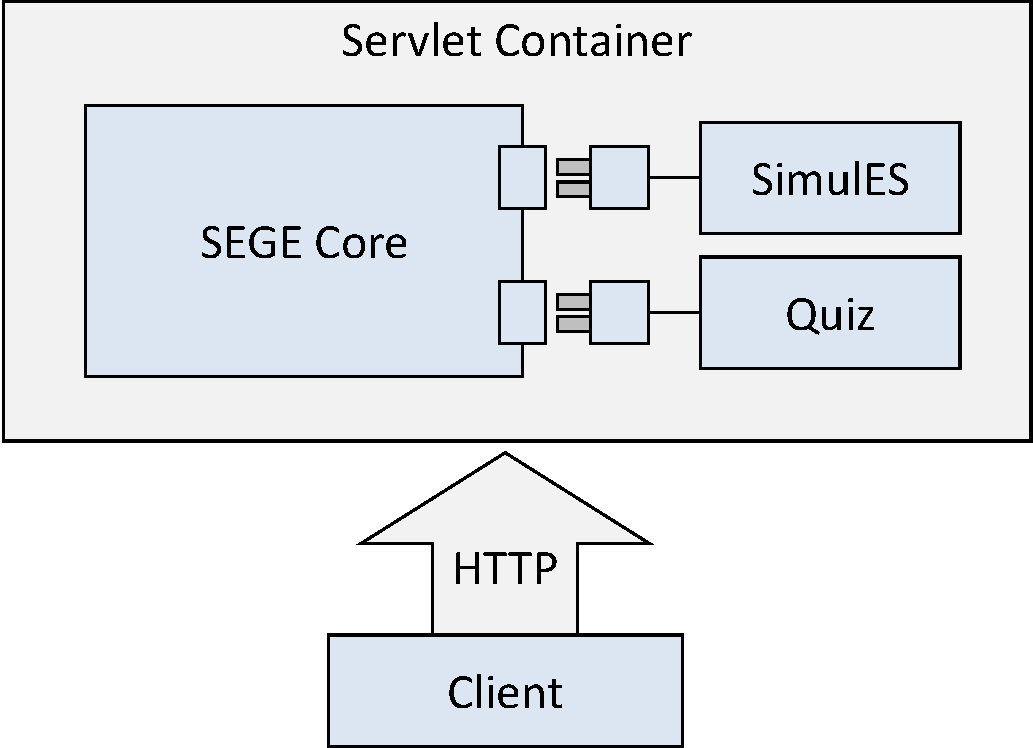
\includegraphics[width=0.5\textwidth]{img/architecture.pdf}
\caption{Arquitetura}
\label{img:architecture}
\end{figure}

Além disso, internamente o serviço utiliza o padrão arquitetural \textbf{microkernel}, onde existe um núcleo mínimo oferecendo um arcabouço geral para implementação dos jogos, mas cada jogo específico é um \emph{plug-in}. Para isso, um jogo deve implementar interfaces básicas exigidas pelo núcleo e deve ser responsável por gerenciar seu estado interno e enumerar as ações disponíveis para os jogadores.


\subsection{Padrões de Projeto}



\section{Instruções de Uso e Exemplos}
\label{sec:examples}



\FloatBarrier
\bibliographystyle{sbc}
\bibliography{bibfile}

\end{document}
